

\section{Introducción}

Para realizar un estudio con mucha estadística de los CRs hasta altas energías se diseñó el Observatorio Pierre Auger. Las propiedades medidas de los lluvias extendidas determinan la energía y la dirección de arribo de cada CR, además de proveer información sobre la distribución de la composición del CR. El Observatorio Pierre Auger en la Provincia de Mendoza, Argentina ha registrado eventos desde el año 2004 mientras se agregaban detectores hasta su terminación en el 2008.

\section{Detección de Rayos Cósmicos}

Una característica esencial del Observatorio es la capacidad de observar lluvias atmosférica extendidas (EAS) simultáneamente mediante dos técnicas distintas, combinando los detectores de superficie (SD) y los detectores de fluorescencia (FD). Los SD son un conjunto de 1660  detectores Cherenkov con agua hiper-pura colocados en un arreglo triangular, con una distancia de $1.5\,$km cubriendo $\sim3000\,$km$^2$, además de un arreglo más pequeño llamado \emph{Infill} separados por $750\,$m. El arreglo principal son los detectores de superficie distanciados 1500\,m, que en el presente trabajo se  referencia como \emph{SD 1500\,m} se muestra en la Fig.\,\ref{fig:auger_sd}. Los FD están colocados en cuatro edificios alrededor del arreglo de SD: Coihueco, Loma Amarilla, Los Morados y Los Leones indicados en el mapa en la Fig.\,\ref{fig:auger_sd}. Cada edificio contiene 6 FD, donde cada uno tiene un campo de visión de $30^o\times30^o$, cubriendo así cada uno $180^o$ en la horizontal.

El área del observatorio es generalmente plana, la altitud de los detectores varía entre $1340\,$m y $1610\,$m, con una altitud media de $\sim1400\,$m. Estos detectores están distribuidos entre las latitudes $35.0^o$ S y $35.3^o$ S y entre las longitudes $69.0^o$ W y $69.4^o$ W.


\subsection{ El detector de superficie y el detector de Fluorescencia}

Un SD consiste en un tanque de polietileno de $3.6\,$m de diámetro que contiene $12\,000$ litros de agua agua hiper-pura. Su interior está recubierto por una lámina de alta reflectividad. En la parte superior se encuentran tres foto-multiplicadores (PMT) distribuidos simétricamente  a $1.2\,$m respecto al centro del tanque. Los mismos colectan la radiación Cherenkov producida por una partícula cargada relativista que pasa por el agua del detector. La altura del tanque de $1.2\,$m lo hace sensible a fotones de altas energías, que pueden convertirse en pares electrón-positrón en el volumen de agua \cite{como_funciona_auger}.

El detector de fluorescencia (FD) consiste en 24 telescopios de fluorescencia, esquematizados en la Fig\,\ref{fig:FD}, distribuidos en 4 distintos lugares en los límite del observatorio. %Estos 4 sitios son: Los Leones, Loma Amarilla, Los Morados y Coihueco, donde 6 de estos telescopios están instalados. 
Cada telescopio tiene un espejo esférico segmentado de 13$\,m^2$ y una cámara que consiste en 440 PMTs ordenados en una grilla de 22x20. Cada telescopio tiene un campo de visión de $30^o\times30^o$.%, por lo tanto cada edificio cubre $180^o$ en acimut.

\begin{figure}[H]
	\centering
	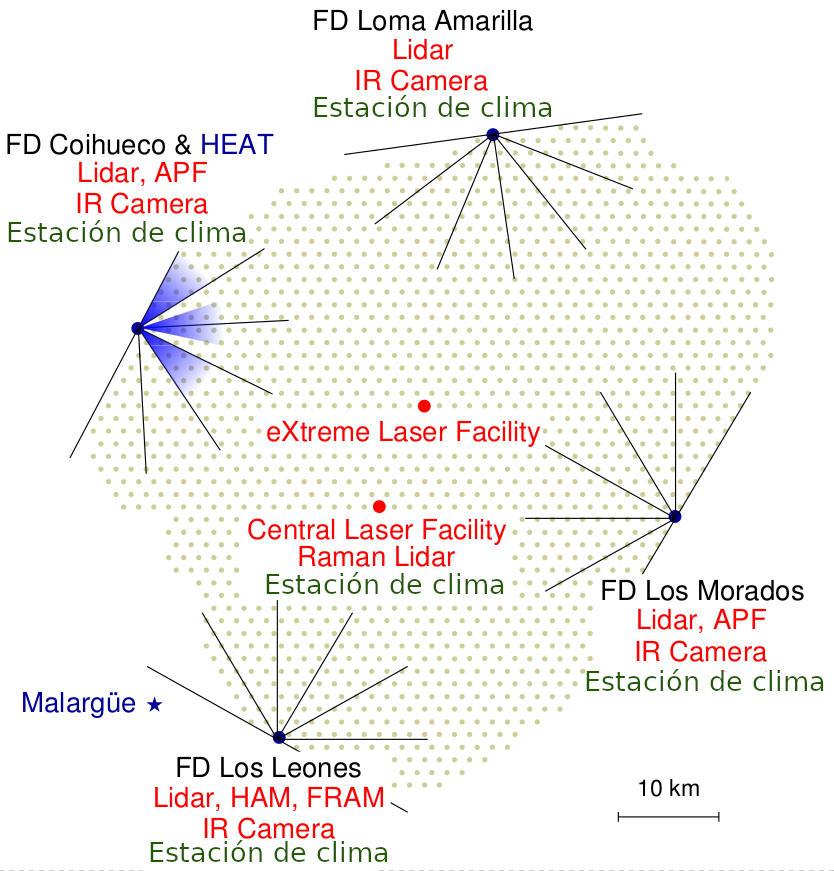
\includegraphics[width=0.75\textwidth]{auger_sd.png}
	\caption{Distribución de los tanques del SD en el área del Observatorio Pierre Auger. Se muestra la ubicación de las estaciones del clima, otros módulos instalados sobre el observatorio y la posición de los detectores de fluorescencia (FD). Figura extraída de \cite{como_funciona_auger}}
	\label{fig:auger_sd}
\end{figure}

\begin{figure}[H]
    \begin{subfigure}[t]{0.45\textwidth}
	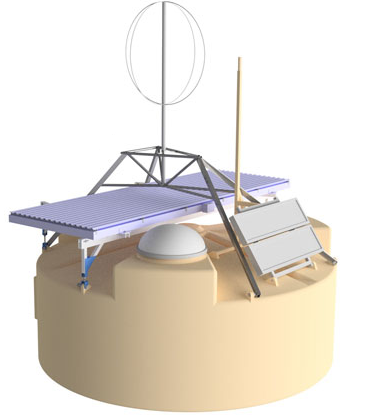
\includegraphics[width=\textwidth]{tanque.png}
	\caption{Detector de radiación Cherenkov con los elementos de la actualización para \emph{Auger Prime}} 	\label{fig:tanque}
    \end{subfigure}%
    \hspace{\fill}
    \begin{subfigure}[t]{0.5\textwidth}
	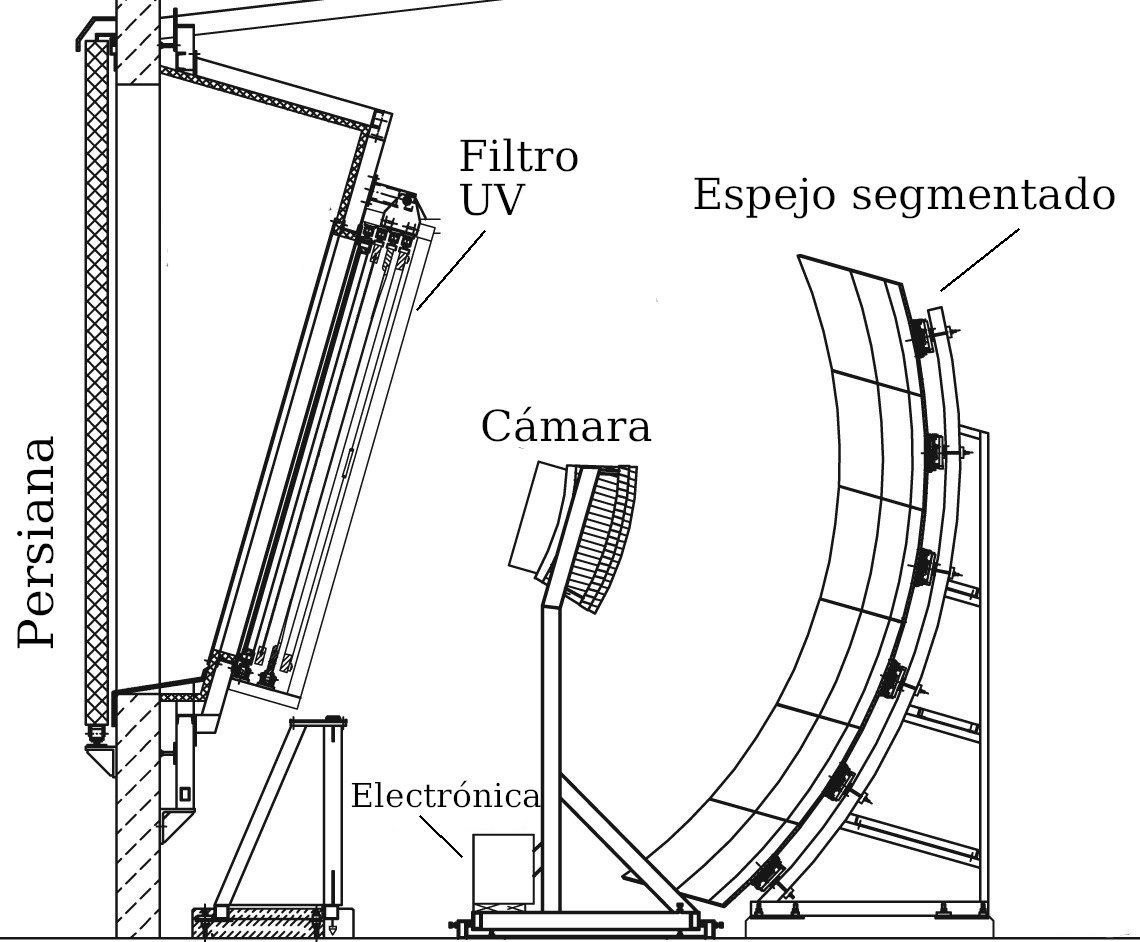
\includegraphics[width=\textwidth]{fd.png}
	\caption{Esquema simplificado de un telescopio de fluorescencia. Extraído de \cite{kit_oracle}}
	\label{fig:FD}
    \end{subfigure}%
    \caption{Detectores empleados por el Observatorio Pierre Auger para la detección de rayos cósmicos.}
	\end{figure}

El FD mide los fotones ultravioletas producidos por la componente electromagnética de la EAS. Mientras se produce la lluvia en la atmósfera, algunos átomos de nitrógeno se excitan y se desexcitan emitiendo fotones. El uso del FD para detectar estos fotones es solo posible en noches sin nubes y sin luna. La posible atenuación de los fotones en la atmósfera es tenida en cuenta para la estimación de energía. Ya que esta estimación se basa en la cantidad de fotones detectados. Otro factor a tener en cuenta es la presencia de aerosoles, como humo o polvo, esto se realiza midiendo la profundidad atmosférica óptica vertical \emph{Vertical Atmosferic Optical Depth (VAOD)}. Estas mediciones son realizadas por los láseres de las instalaciones de Central Laser Facility (CLF) y de eXtreme Laser Facility (XLF), cuyas ubicaciones se muestra en la Fig.\ref{fig:auger_sd}.

\subsection{Diseño híbrido}\label{seccion:sd_eff}

El SD detecta un corte de EAS que llega al nivel del suelo, los WCDs detectan la componentes electromagnética y muónica de la lluvia. Cabe resaltar que el SD funciona las 24 horas del día, por lo que detecta una mayor cantidad de eventos que el FD. Existen métodos para determinar la dirección de arribo y la energía del primario.  La exposición se calcula contando la cantidad de hexágonos activos en un tiempo dado, y multiplicado la apertura de una sola celda hexagonal que vale $4.59\,$km$^2$.sr para lluvias verticales. El SD tiene la propiedad de que la calidad de sus mediciones aumenta con la energía del EAS. La exposición instantánea del SD se calcula fácilmente, especialmente para energías mayores a 3 EeV, donde la EAS detectada por cualquier parte del SD es detectada con 100\% de eficiencia independientemente de la masa del primario que inicio la EAS.

El FD es usado para generar una imagen del desarrollo del EAS en la atmósfera. La luz de fluorescencia es emitida isotrópicamente en la parte ultravioleta del espectro, y es producida predominantemente por la componente electromagnética de la lluvia. Los períodos de observación están limitados a las noches sin luna y con buen clima, pero la ventaja del FD es la posibilidad de ver el desarrollo de la lluvia. Dado que la producción de la fotones por fotoluminiscencia es proporcional a la energía depositada en la atmósfera, se puede medir la energía del primario mediante calorimetría. Otro aspecto importante del FD es la posibilidad de medir la profundidad de la atmósfera donde la lluvia alcanza su máximo desarrollo, $X_{max}$, esta cantidad es uno de los más directos indicadores de la composición de masa. \cite{data}

\section{Reconstrucción de eventos de los detectores  de superficie}

\subsection{Selección de eventos}

La reconstrucción de la energía y la dirección de arribo de los CRs se realiza mediante las señales medidas por el SD. La dirección es reconstruida mediante  el tiempo de llegada de las señales registradas por estaciones individuales del SD. Para garantizar la selección de eventos bien contenidos en el SD, se aplica el corte llamado \emph{6T5}. Este corte considera solo a los eventos donde el tanque con mayor señal está rodeado por otros 6 tanques activos. Esta condición asegura una buena reconstrucción de la energía. Al mismo tiempo, este corte simplifica el cálculo de la exposición \cite{exposure}, importante  para el análisis del espectro. Para estudios de dirección de arribo pueden utilizar cortes menos estrictos.

\subsection{Reconstrucción de las lluvias}

En una primera aproximación para la dirección de arribo de la lluvia se obtiene ajustando los tiempos de llegada de la señal en cada tanque. Para eventos con suficientes tanques disparados, estos tiempos de llegada pueden ser descritas como la evolución un frente de lluvia como una esfera que crece con la velocidad de la luz. Los puntos de impacto del EAS con el suelo son obtenidas mediante ajustes a las señales de los tanques. Este ajuste se realiza con un función de distribución lateral (LDF). La LDF también tiene en cuenta la probabilidad de que los tanques no sean disparados y que los tanques con mayor señal estén saturados.

Un ejemplo de la señal que deja un evento sobre el SD 1500 m se muestra en la Fig.\,\ref{fig:evento_sd}. Este evento fue producido por un rayo cósmico de ($104\pm11$)\,EeV con un ángulo cenital de ($25.1\pm0.1 ^o$). La LDF de las señales para este evento se muestra en la Fig.\,\ref{fig:evento_S1000}. La función utilizada para el ajuste de la LDF es una función  $f_{LDF}$ propuesta por Nishimura-Kamata-Greisen \cite{data}
\begin{align*}
	%S(r) = S(r_{opt})\bigg(\frac{r}{r_{opt}}\bigg)^{\beta}\bigg(\frac{r+r_1}{r_{opt}+r_1}\bigg)^{\beta + \gamma}
	S(r) &= S(r_{opt})f_{LDF}(r)\\
	f_{LDF}(r)&=\bigg(\frac{r}{r_{opt}}\bigg)^{\beta}\bigg(\frac{r+r_1}{r_{opt}+r_1}\bigg)^{\beta + \gamma}
\end{align*}
donde $f_{LDF}$ está normalizado tal que $f_{LDF}(r_{opt})=1$ y $r_{opt}$ es la distancia óptima, %$r_1=700\,$m 
y $S(r_{opt})$ es usado para estimar la energía. Para el arreglo SD 1500\,m, el parámetro $r_{opt}=1000\,$m, por lo tanto el tamaño de la lluvia o \emph{shower size} es el valor de S(1000). Dado que la forma de la LDF es desconocida, la forma funcional propuesta para la función $f_{LDF}$ fue elegida empíricamente.  El parámetro $\beta$ depende del tamaño de la lluvia y del ángulo cenital. Los eventos verticales, es decir los eventos con $\theta < 60^o$, son medidas en una etapa menos desarrollada que eventos más inclinados. Los eventos con $\theta>60^o$ atraviesan un mayor cantidad de atmósfera.


\begin{figure}[H]
	\begin{small}
		\begin{center}
			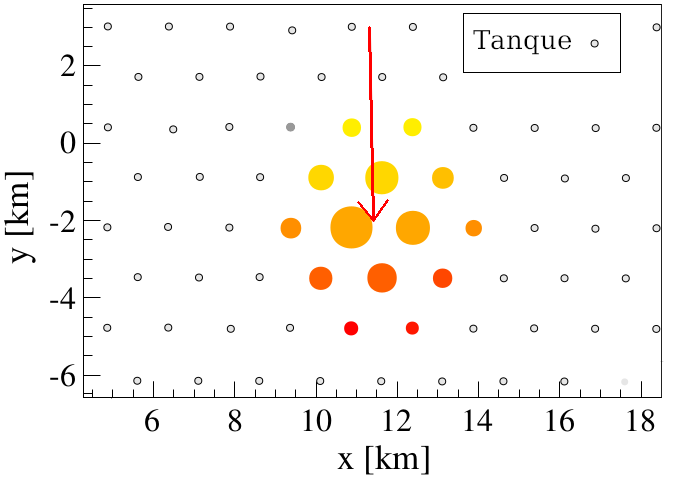
\includegraphics[width=0.65\textwidth]{evento_sd.png}
		\end{center}
		\caption{Ejemplo de la señal dejada por un evento de ($104\pm11$)\,EeV de energía con un ángulo cenital de ($25.1\pm0.1 ^o$) sobre el arreglo principal SD 1500 m. La flecha indica la dirección de arribo de la lluvia. Los colores de los círculo representa el tiempo de arribo de la lluvia, los primeros en amarillo y los últimos en rojo. En área de los círculo pintados es proporcional a logaritmo de la señal. Figura extraída de \cite{como_funciona_auger}. } 	\label{fig:evento_sd}
	\end{small}
\end{figure}


\begin{figure}[H]
	\begin{small}
		\begin{center}
			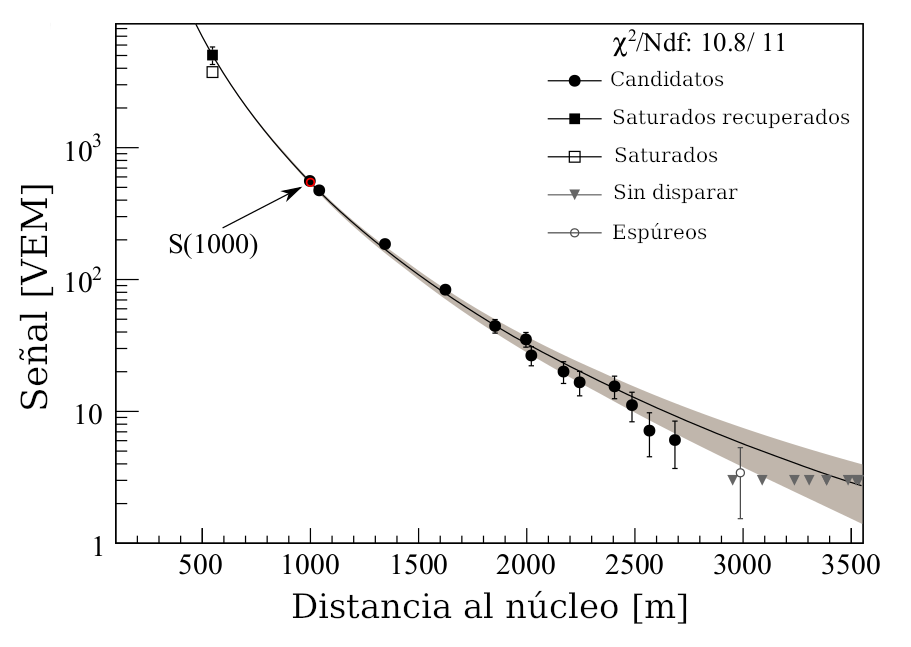
\includegraphics[width=0.65\textwidth]{evento_s1000.png}
		\end{center}
		\caption{Dependencia de la señal con la distancia del núcleo de la lluvia de un evento de ($104\pm11$)\,EeV de energía con un ángulo cenital de ($25.1\pm0.1 ^o$). La función ajustada es la función de distribución lateral (LDF). Del ajuste se obtiene el valor de S(1000). Figura extraída de \cite{como_funciona_auger}. } 	\label{fig:evento_S1000}
	\end{small}
\end{figure}


\subsection{Calibración de la energía}

Para una energía dada, el valor de S(1000) disminuye con $\theta$ debido a la atenuación de las partículas de la lluvia. Asumiendo un flujo isotrópico de los CR primarios sobre la parte superior de la atmósfera, se obtiene la atenuación de los datos mostrados en la Fig.\,\ref{fig:s1000_theta}  usando el método de Corte de Intensidad Constante (CIC) \cite{CIC}. La curva de atenuación $f_{CIC}(\theta)$ fue ajustado con un polinomio de orden 3 del tipo $f_{CIC}(\theta)=1+ax+bx^2+cx^3$, donde $x=\cos^2(\theta) - \cos^2(38^o)$. Según lo presentado por la colaboración \cite{collaboration2013pierre}, los valores son $a=0.980\pm0.004$, $b=-1.68\pm0.01$ y $c=-1.30\pm 0.45$, aunque estos coeficientes cambian ligeramente con la energía \cite{data}. El ángulo cenital $\theta=38^o$ se toma como un punto de referencia para convertir S(1000) a S$_{38}$ mediante $S_{38}=S(1000)/f_{CIC}(\theta)$. Este valor S$_{38}$ puede considerarse como la señal S(1000) que hubiera tenido un evento que fue detectado mediante el SD con $\theta=38^o$.

Los eventos con $\theta<60^o$  que fueron detectados por el SD y por el FD son utilizados para relacionar el tamaño de la lluvia con la energía  E$_{FD}$ medida por calorimetría por el FD.  La correlación entre S$_{38}$ y E$_{FD}$ se calcula mediante el método de máxima verosimilitud, que considera la evolución de las incertezas con la energía. La relación entre S$_{38}$ y $E_{FD}$ se describe mediante un función de potencia como se muestra en la Ec.\,\ref{eq:s38_energy}
\begin{equation}
	E_{FD}= A\, (S_{38}/VEM)^B
	\label{eq:s38_energy}
\end{equation}
donde los parámetros obtenidos son $A=(1.86\pm0.03)\times 10^{17}\,$eV y $B=(1.031\pm0.004)$  \cite{tobepublished}. En la Fig.\,\ref{fig:efd_s38} se observa el ajuste y la relación entre  S$_{38}$ y E$_{FD}$


\begin{figure}[H]
    \begin{subfigure}[t]{0.51\textwidth}
	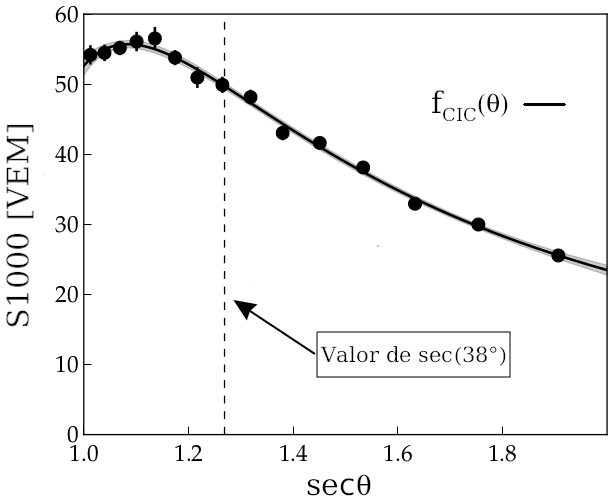
\includegraphics[width=\textwidth]{s1000_theta.png}
	\caption{Curva de atenuación descrita por un polinomio de orden 3. En este ejemplo se deducen los coeficientes de la dependencia del S(1000) a S$_{38}\approx 50\,$VEM que corresponde a un energía de $10.5\,$EeV.} 	\label{fig:s1000_theta}
    \end{subfigure}%
    \hspace{\fill}
    \begin{subfigure}[t]{0.45\textwidth}
	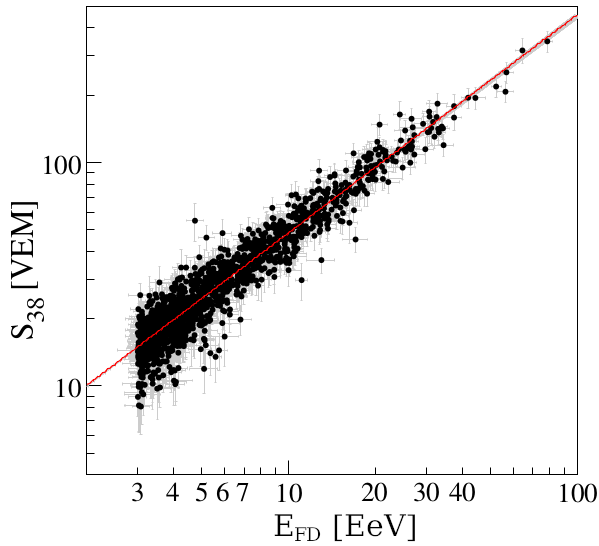
\includegraphics[width=\textwidth]{efd_s38.png}
	\caption{Correlación entre el valor S$_{38}$ y la energía $E_{FD}$ medida por el FD.} 	\label{fig:efd_s38}
    \end{subfigure}%
    \caption{Distintas calibraciones hechas para los eventos reconstruidos en el Observatorio Pierre Auger.}
	\end{figure}



\subsection{Monitoreo del clima}\label{seccion:clima}

Las condiciones atmosféricas, como la temperatura, presión y humedad, se deben tener en cuenta para estudiar el desarrollo de los EAS, así como también para estudiar la cantidad de fotones de las lluvias sobre los moléculas de N$_2$, emitidos por fluorescencia. Distintas estaciones monitorean las condiciones atmosféricas sobre el Observatorio Pierre Auger, cuatro cerca  de los edificios donde se encuentran los FD y uno cerca del centro del SD 1500\,m. Para este trabajo se utilizaron las mediciones de la presión y temperatura registradas la mayor parte del tiempo en la estación del clima cerca del CLF, la misma realiza una medición cada intervalo de 5 minutos la mayor parte del tiempo. Cuando no se cuenta con datos registrados para intervalos entre 10 minutos hasta 3 horas, en estos casos se utiliza una interpolación de los datos medidos. Si el período de tiempo es mayor a 3 horas, los eventos durante este periodo no son considerados para la determinación de los efectos del clima en la señal detectada por el SD 1500\,m.